\documentclass{article}
\usepackage{graphicx} % Required for inserting images
\usepackage[hungarian]{babel}
\usepackage{hulipsum}
\usepackage{subcaption}
\usepackage{array}
\usepackage[table]{xcolor}
\usepackage{multirow,multicol}
\usepackage{wrapfig}
\usepackage{listings}
\usepackage{float}

\floatstyle{plain}
\newfloat{PythonCode}{H}{lop}[section]
\newfloat{CCode}{H}{loc}[section]
\floatname{PythonCode}{Python Kód}
\floatname{CCode}{C Kód}


\definecolor{hatter}{rgb}{0.95, 0.95, 0.95}
\definecolor{kulcs}{rgb}{0.6, 0.1, 0.1}
\definecolor{fugveny}{rgb}{0.0, 0.0, 0.5}
\definecolor{komment}{rgb}{0.4, 0.4, 0.4}


\lstdefinestyle{egyediPython}{
    language=Python,
    tabsize=2,
    showtabs=false,
    showspaces=false,
    frame=single,
    numbers=left,
    stepnumber=4,
    xleftmargin=10pt,
    numbersep=5pt,
    framesep=20pt
}


\lstdefinestyle{egyediC}{
    language=C,
    backgroundcolor=\color{hatter},
    keywordstyle=\color{kulcs},
    identifierstyle=\color{fugveny},
    commentstyle=\color{komment},
    tabsize=2,
    showspaces=false,
    showtabs=false,
    numbers=left,
    stepnumber=3,
    numbersep=5pt,
    frame=none,
    breaklines=true,
}

\title{Készfeladat03.01}
\author{Viktor Soltész}
\date{November 2024}

\begin{document}

\maketitle

\section{Introduction}
\listoffigures
\listoftables
\hulipsum

\includegraphics[keepaspectratio,width=5cm]{szines.jpg}
\hulipsum[2-5]

\begin{figure}
    \centering
    \begin{subfigure}[t]{0.45\linewidth}
        \centering
        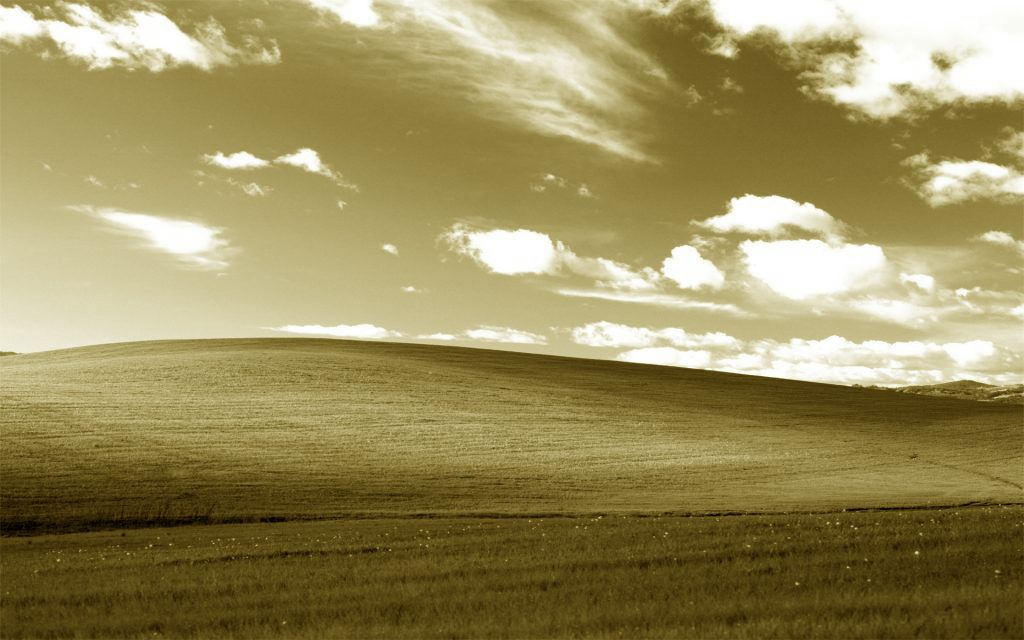
\includegraphics[width=\linewidth]{szepia.jpg}
        \caption{1. részábra}
        \label{fig:subfig1}
    \end{subfigure}
    \begin{subfigure}[t]{0.45\linewidth}
        \centering
        \reflectbox{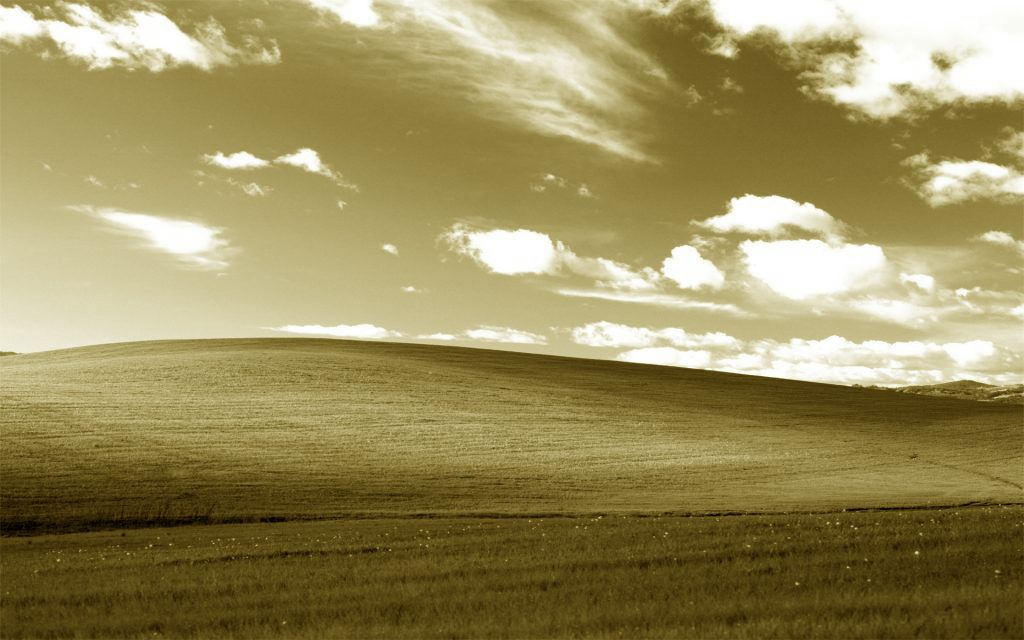
\includegraphics[width=\linewidth]{szepia.jpg}}
        \caption{2. részábra tükrözve}
        \label{fig:subfig2}
    \end{subfigure}
    
    \caption{Fő ábra}
    \label{fig:mainfigure}
\end{figure}
\hulipsum[2-5]

\begin{table}
    \centering
    \caption{1. táblázat}
    \begin{tabular}{|m{30pt}||l|c|r|}
        \hline
         & egy & kettő & három \\ \hline
        Helló világ & négy & öt & hat \\ \hline
         & hét & nyolc & kilenc \\ \hline
        lórumipse& tíz & & tizenkettő \\ \hline
    \end{tabular}
    \label{tab:table1}
\end{table}
\hulipsum[3]

\begin{table}
    \centering
    \caption{2. táblázat}
    \rowcolors[\hline]{2}{blue!20}{yellow!20}
    \begin{tabular}{|l|c|r|}
        \hline
        egy & kettő & három \\ \hline
        négy & öt & hat \\ \hline
        hét & nyolc & kilenc \\ \hline
        tíz & & tizenkettő \\ \hline
    \end{tabular}
    \label{tab:table2}
\end{table}
\hulipsum[2]

\begin{wraptable}[12]{r}[\marginparwidth]{5cm}
    \centering
    \caption{3. táblázat}
    \begin{tabular}{|l|c|r|}
        \hline
        egy&\multicolumn{2}{|c|}{kettő}\\ \hline
        \multirow{2}{*}{négy} & öt & hat \\ \hline
        & \multicolumn{2}{|c|}{\multirow{2}{*}{nyolc}} \\ \hline
        tíz & &  \\ \hline
    \end{tabular}
    \label{tab:table3}
\end{wraptable}

\begin{table}
    \centering
    \caption{4. táblázat}
    \begin{tabular}{|l|c|r|}
        \hline
        egy&\multicolumn{2}{|c|}{kettő}\\ \hline
        \multirow{2}{*}{négy} & öt & hat \\ \hline
        & \multicolumn{2}{|c|}{\multirow{2}{*}{nyolc}} \\ \hline
        tíz & &  \\ \hline
    \end{tabular}
    \label{tab:table4}
\end{table}

3-as feladat \verb|\LaTeX| a része \verb|\begin{document}| inline verbatim használata.

\begin{verbatim}
\begin{table}
    \centering
    \caption{2. táblázat}
    \rowcolors[\hline]{2}{blue!20}{yellow!20}
    \begin{tabular}{|l|c|r|}
        \hline
        egy & kettő & három \\ \hline
        négy & öt & hat \\ \hline
        hét & nyolc & kilenc \\ \hline
        tíz & & tizenkettő \\ \hline
    \end{tabular}
    \label{tab:table2}
\end{table}
\end{verbatim}

\clearpage

\begin{lstlisting}
def binary_search(arr, val, start, end):
	if start == end:
		if arr[start] > val:
			return start
		else:
			return start+1
	elif start > end:
		return start
	else: 
		mid = (start+end)/2
		if arr[mid] < val:
			return binary_search(arr, val, mid+1, end)
		elif arr[mid] > val:
			return binary_search(arr, val, start, mid-1)
		else: # arr[mid] = val
			return mid
			
def insertion_sort(arr):
    for i in xrange(1, len(arr)):
        val = arr[i]
        j = binary_search(arr, val, 0, i-1)
        arr = arr[:j] + [val] + arr[j:i] + arr[i+1:]
    return arr
\end{lstlisting}

\begin{lstlisting}[style=egyediPython, caption={Python példa kód}]
def binary_search(arr, val, start, end):
    if start == end:
        if arr[start] > val:
            return start
        else:
            return start+1
    elif start > end:
        return start
    else: 
        mid = (start+end) // 2
        if arr[mid] < val:
            return binary_search(arr, val, mid+1, end)
        elif arr[mid] > val:
            return binary_search(arr, val, start, mid-1)
        else: # arr[mid] = val
            return mid
\end{lstlisting}

\begin{CCode}
\centering
\lstinputlisting[style=egyediC, caption={C kód: Első függvény}, firstline=10, lastline=20]{binsearch.c}
\end{CCode}

\begin{CCode}
\centering
\lstinputlisting[style=egyediC, caption={C kód: Második függvény}, firstline=5, lastline=10]{binsearch.c}
\end{CCode}

\end{document}
